%%%%%%%%%%%%%%%%%%%%%%%%%%%%%%%%%%%%%%%%%%%%%%%%%%%%%%%%%%%%%%%%%%%%%%%%%%%%%%%%%%%%%%%%%%%%%%%%%%%%%%%%%%%%%%%%
%BESCHREIBUNG
%%%%%%%%%%%%%%%%%%%%%%%%%%%%%%%%%%%%%%%%%%%%%%%%%%%%%%%%%%%%%%%%%%%%%%%%%%%%%%%%%%%%%%%%%%%%%%%%%%%%%%%%%%%%%%%%
%Autor (Vorlage): Janik Siller
%Created: 07/2018
%
% !TeX root = Projektarbeit.tex
%
%LaTeX Formatvorlage für wissenschaftliche Arbeiten
%
%Empfohlene LaTeX Distribution: TeXLive; 
%	Available: https://www.tug.org/texlive/
%Empfohlener Editor: Visual Studio Code; 
%	Available: https://code.visualstudio.com/
%Empfohlenes LaTeX Plugin für VS Code: LaTeX Workshop; 
%	Available: https://marketplace.visualstudio.com/items?itemName=James-Yu.latex-workshop
%
%Version: 2.0.2
%%%%%%%%%%%%%%%%%%%%%%%%%%%%%%%%%%%%%%%%%%%%%%%%%%%%%%%%%%%%%%%%%%%%%%%%%%%%%%%%%%%%%%%%%%%%%%%%%%%%%%%%%%%%%%%%

%%%%%%%%%%%%%%%%%%%%%%%%%%%%%%%%%%%%%%%%%%%%%%%%%%%%%%%%%%%%%%%%%%%%%%%%%%%%%%%%%%%%%%%%%%%%%%%%%%%%%%%%%%%%%%%%
%PRÄAMBEL
%%%%%%%%%%%%%%%%%%%%%%%%%%%%%%%%%%%%%%%%%%%%%%%%%%%%%%%%%%%%%%%%%%%%%%%%%%%%%%%%%%%%%%%%%%%%%%%%%%%%%%%%%%%%%%%%
\documentclass[
	pdftex,	
	a4paper,
	12pt,
	parskip = half,
	listof=totoc,
	bibliography=totoc,
    headheight = 50pt]
	{scrartcl}


% Sprachpaket Deutsch ------------------------------------------------------------------------------------------
\usepackage[ngerman]{babel}
% UTF8 und T1 Fontencoding -------------------------------------------------------------------------------------


\usepackage{csquotes}

\usepackage[backend=biber,style=alphabetic]{biblatex}

\addbibresource{content/literature.bib}

\usepackage[T1]{fontenc}
% ToDo Notes ---------------------------------------------------------------------------------------------------
%\usepackage{todonotes}
% Kopf / Fußzeilen----------------------------------------------------------------------------------------------
\usepackage[headsepline, footsepline]{scrlayer-scrpage}
% Grafiken einbinden--------------------------------------------------------------------------------------------
\usepackage{graphicx}

% Einfache Verwendung von Farben -------------------------------------------------------------------------------
\usepackage{xcolor}
% Inhaltsverzeichnis als Lesezeichen in PDF --------------------------------------------------------------------
\usepackage{hyperref}
\hypersetup{hidelinks}
% Seitenränder -------------------------------------------------------------------------------------------------
\usepackage[left = 25mm, right=25mm, top=35mm, bottom=30mm, head=41pt]{geometry}
% Zeilenabstand ------------------------------------------------------------------------------------------------
\usepackage{setspace}
% Abkürzungen, Abkürzungsverzeichnis ---------------------------------------------------------------------------
\usepackage{acronym}
% Fixe Positionierung von Bildern mit der Option [H]------------------------------------------------------------
\usepackage{here}
% Latin Modern Schriftart - schönere Darstellung in PDF --------------------------------------------------------
\usepackage{lmodern}
% Mehr Darstellungsoptionen bei Aufzählungen -------------------------------------------------------------------
\usepackage{enumitem}
% Ermöglicht Berechnungen in den Argumenten von Kommandos ------------------------------------------------------
\usepackage{calc}
% Darstellung von Geburt und Tod -------------------------------------------------------------------------------
\usepackage{textcomp}
% Bessere Zeilentrennung zur Vermeidung von overful hbox -------------------------------------------------------
%\usepackage{microtype}
% AMS Mathematikpake--------------------------------------------------------------------------------------------
\usepackage{amsmath}
% Quellcodelistings --------------------------------------------------------------------------------------------
\usepackage{listings}
\usepackage{wrapfig}
\usepackage{textcomp}
\usepackage{textgreek}

%%%%%%%%%%%%%%%%%%%%%%%%%%%%%%%%%%%%%%%%%%%%%%%%%%%%%%%%%%%%%%%%%%%%%%%%%%%%%%%%%%%%%%%%%%%%%%%%%%%%%%%%%%%%%%%%
%META INFORMATIONEN
%%%%%%%%%%%%%%%%%%%%%%%%%%%%%%%%%%%%%%%%%%%%%%%%%%%%%%%%%%%%%%%%%%%%%%%%%%%%%%%%%%%%%%%%%%%%%%%%%%%%%%%%%%%%%%%%
% Projektspezifische Informationen -----------------------------------------------------------------------------
\newcommand{\titel}{Nutzung von Künstlichen Intelligenzen zur Realisierung eines Intelligenten Fehlersupports}
\newcommand{\arbeit}{Prüfungsabgabe im Fach Automatisierung}
\newcommand{\studiengang}{Elektro- und Informationstechnik,\\Automation}
\newcommand{\hochschule}{DHBW Ravensburg}
\newcommand{\campus}{Campus Friedrichshafen}
\newcommand{\autor}{Thomas Martin}
\newcommand{\abgabe}{18.12.2026}
\newcommand{\zeitraum}{30.09.2026 - 18.12.2026}
\newcommand{\matrikelnummer}{2566504}
\newcommand{\unternehmen}{RAFI GmbH \& Co. KG}
\newcommand{\unternehmenstr}{Ravensburger Str. 128-134}
\newcommand{\unternehmenaddr}{88276 Berg}
\newcommand{\betreuereins}{}
\newcommand{\betreuerzwei}{}
\newcommand{\betreuerdrei}{}
%\newcommand{\gutachter}{Prof. Dr. Gutachter}
\newcommand{\ort}{Berg}
% Information für PDF Generierung ------------------------------------------------------------------------------
\hypersetup{
	pdftitle = {\titel},
	pdfsubject = {\titel},
	pdfauthor = {\autor}
}

%%%%%%%%%%%%%%%%%%%%%%%%%%%%%%%%%%%%%%%%%%%%%%%%%%%%%%%%%%%%%%%%%%%%%%%%%%%%%%%%%%%%%%%%%%%%%%%%%%%%%%%%%%%%%%%%
%LAYOUT
%%%%%%%%%%%%%%%%%%%%%%%%%%%%%%%%%%%%%%%%%%%%%%%%%%%%%%%%%%%%%%%%%%%%%%%%%%%%%%%%%%%%%%%%%%%%%%%%%%%%%%%%%%%%%%%%
%Kopf- und Fußzeilen -------------------------------------------------------------------------------------------
\pagestyle{scrheadings}
\clearpairofpagestyles
\ihead{
\includegraphics[height = 1.25 cm]{logos/logo_dhbw.png}}
\ohead{
\includegraphics[height = 0.65 cm]{logos/logo_rafi.png}}
\ofoot{\pagemark}
%Anpassen der KOMA Überschriften -------------------------------------------------------------------------------
\addtokomafont{sectioning}{\rmfamily}
%Zeilenabstand--------------------------------------------------------------------------------------------------
\onehalfspacing
%Counter für römische Seitenzahl -------------------------------------------------------------------------------
\newcounter{savepage}
%Quellenangabe von Grafiken ------------------------------------------------------------------------------------
\newcommand*{\quelle}[1]{\footnotesize ~#1}
%Größe von Abbildungen------------------------------------------------------------------------------------------
\newcommand{\imgsmall}{0.25\textwidth}
\newcommand{\imgmedium}{0.5\textwidth}
\newcommand{\imgbig}{0.75\textwidth}
\newcommand{\imglarge}{\textwidth}
%Quellcodeformatierung -----------------------------------------------------------------------------------------

%Farben------------------------------------
\colorlet{punct}{red!60!black}
\definecolor{background}{HTML}{EEEEEE}
\definecolor{delim}{RGB}{20,105,176}
\colorlet{numb}{magenta!60!black}
\definecolor{deepblue}{rgb}{0,0,0.5}
\definecolor{deepred}{rgb}{0.6,0,0}
\definecolor{deepgreen}{rgb}{0,0.5,0}

\DeclareFixedFont{\ttb}{T1}{txtt}{bx}{n}{8} % for bold
\DeclareFixedFont{\ttm}{T1}{txtt}{m}{n}{8}  % for normal

%JSON -------------------------------------
\lstdefinelanguage{json}{
	basicstyle=\scriptsize\normalfont\ttfamily,
    numbersep=8pt,
	showstringspaces=false,
	captionpos=b,
    breaklines=true,
    frame=lines,
    backgroundcolor=\color{background},
    literate=
     *{0}{{{\color{numb}0}}}{1}
      {1}{{{\color{numb}1}}}{1}
      {2}{{{\color{numb}2}}}{1}
      {3}{{{\color{numb}3}}}{1}
      {4}{{{\color{numb}4}}}{1}
      {5}{{{\color{numb}5}}}{1}
      {6}{{{\color{numb}6}}}{1}
      {7}{{{\color{numb}7}}}{1}
      {8}{{{\color{numb}8}}}{1}
      {9}{{{\color{numb}9}}}{1}
      {:}{{{\color{punct}{:}}}}{1}
      {,}{{{\color{punct}{,}}}}{1}
      {\{}{{{\color{delim}{\{}}}}{1}
      {\}}{{{\color{delim}{\}}}}}{1}
      {[}{{{\color{delim}{[}}}}{1}
      {]}{{{\color{delim}{]}}}}{1},
}

%Python -------------------------------------
\newcommand\pythonstyle{\lstset{
    basicstyle=\scriptsize\normalfont\ttfamily,
    showstringspaces=false,
    language=Python,
	captionpos=b,
    breaklines=true,
    frame=lines,
    backgroundcolor=\color{background},
    otherkeywords={self},             % Add keywords here
    keywordstyle=\ttb\color{deepblue},
    emph={MyClass,__init__},          % Custom highlighting
    emphstyle=\ttb\color{deepred},    % Custom highlighting style
    stringstyle=\color{deepgreen},
    frame=tb                        % Any extra options here
}}

\lstnewenvironment{python}[1][]
{
\pythonstyle
\lstset{#1}
}
{}

%%%%%%%%%%%%%%%%%%%%%%%%%%%%%%%%%%%%%%%%%%%%%%%%%%%%%%%%%%%%%%%%%%%%%%%%%%%%%%%%%%%%%%%%%%%%%%%%%%%%%%%%%%%%%%%%
%HAUPTTEIL
%%%%%%%%%%%%%%%%%%%%%%%%%%%%%%%%%%%%%%%%%%%%%%%%%%%%%%%%%%%%%%%%%%%%%%%%%%%%%%%%%%%%%%%%%%%%%%%%%%%%%%%%%%%%%%%%

\begin{document}

    % Deckblatt ----------------------------------------------------------------------------------------------------
    \begin{titlepage}
	\vspace*{-\topskip}\vspace*{-\headsep}\vspace{-14mm}

	\begin{minipage}[c]{0.23\textwidth} 
    	
\includegraphics[height=1.25 cm]{logos/logo_dhbw.png} 
  	\end{minipage}
  	\hfill 
  	\begin{minipage}[c]{0.28\textwidth} 
    	 
\includegraphics[height=0.65 cm]{logos/logo_rafi.png}
  	\end{minipage}	
	
	\vspace{\headsep}\vspace{\topskip}
	
	\begin{center}		
		{\large \bfseries \titel}
		\vfill
		{\bfseries \arbeit}
		\vfill
		im Studiengang \studiengang
		\vfill
		an der \hochschule \\
		\campus
		\vfill
		von 
		\vfill
		\autor 
		\vfill
		\abgabe
		\vfill
	\end{center}
	
	\begin{tabular}{l l }
		Bearbeitungszeitraum: & \zeitraum \\
		Matrikelnummer: &    \matrikelnummer \\
	%	Gutachter der Dualen Hochschule: & \gutachter \\
	
	\end{tabular}
	
\end{titlepage}

    % Eidesstattliche Erklärung-------------------------------------------------------------------------------------
    \newpage
    \pagenumbering{Roman}
    \section*{Eidesstattliche Erklärung} 


gemäß Ziffer 1.1.13 der Anlage 1 zu §§ 3, 4 und 5  der Studien- und Prüfungsordnung für die Bachelorstudiengänge 
im Studienbereich Technik der Dualen Hochschule Baden-Württemberg vom 29.09.2017 in der Fassung vom 25.07.2018.

Ich versichere hiermit, dass ich meine Projektarbeit mit dem Thema:
\begin{center}
{\bfseries \titel}
\end{center}
selbstständig verfasst und keine anderen als die angegebenen Quellen und Hilfsmittel benutzt habe. Ich 
versichere zudem, dass die eingereichte elektronische Fassung mit der gedruckten Fassung übereinstimmt.

\ort , den \abgabe .

\begin{tabular}{l}
\\
\\ \cline{1-1} 
{\footnotesize \autor} \hspace{15mm} \\

\end{tabular}

    % Sperrvermerk ------------------------------------------------------------------------------------------------
    %\newpage
    %\input{content/0_0_3Sperrvermerk.tex}

    %Leitgedanke ---------------------------------------------------------------------------------------------------
    %\newpage
    %\input{content/0_0_4Leitgedanke.tex}

    %Kurzbeschreibung-----------------------------------------------------------------------------------------------
    %\newpage
    %\input{content/0_0_5Kurzbeschreibung.tex}

    %Abstract-------------------------------------------------------------------------------------------------------
    %\newpage
    %\input{content/0_0_6Abstract.tex}

    %Danksagung-----------------------------------------------------------------------------------------------------
    %\newpage
    %\input{content/0_0_7Danksagung.tex}

    %Inhaltsverzeichnis---------------------------------------------------------------------------------------------
    \newpage
    \tableofcontents
    
    \setcounter{savepage}{\value{page}}
    \newpage

    %Beginn der Hauptkapitel-----------------------------------------------------------------------------------------------------
    \pagenumbering{arabic}
    \section{Einleitung}
    In der industriellen Fertigung setzt die RAFI Gruppe auf hochautomatisierte Produktionsanlagen, um Produkte personalunabhängig, in gleichbleibend hoher Qualität und unter maximaler Wirtschaftlichkeit herzustellen. Als Steuerungsbasis kommen vor allem Industrie-PCs des Herstellers Beckhoff in den Produktionsanlagen zum Einsatz.


\subsection{Ausgangszustand} 

    Kommt es zu einem Anlagenfehler, wird die Produktion unterbrochen, bis das Instandhaltungspersonal die Anlage wieder in einen funktionsfähigen Zustand versetzt hat. Da während dieser Stillstandszeit keine Produkte gefertigt werden können, entstehen erhebliche Opportunitätskosten. Um diese Ausfallzeiten so gering wie möglich zu halten, ist im Fehlerfall eine schnelle und zielgerichtete Ursacheneingrenzung entscheidend. Durch eine rasche Wiederaufnahme der Produktion profitiert RAFI von minimalen Stillstandszeiten und einer effizienteren Arbeitsweise des Wartungspersonals. Bislang ist das Personal bei der Störungsbehebung jedoch auf sich allein gestellt und muss ohne vorgefertigte Hilfsmittel arbeiten, was den Prozess kompliziert und untranstransparent macht und ein zielstrebiges Vorgehen erschwert. Genau an dieser Herausforderung setzt das genannte Problem an:
    
    

\subsection{Problemdefinition}

    Die Instandsetzung der Anlage ist nicht nur sehr zeitintensiv, sondern dadurch auch mit hohen Kosten verbunden. Der Hauptgrund für die langen Ausfallzeiten liegt darin, dass das Wartungspersonal bisher keine strukturierten Informationen zum Zustand der Anlage vor einem Anlagenfehler erhält. Man kann also keine Fehlerursache ableiten. Die einsehbaren Variablen und Programmzustände sind unübersichtlich, wodurch die Auswertung komplex, zeitaufwendig und fehleranfällig wird. Konkret fehlen dem Personal wichtige Daten zu aktiven Anlagenzuständen oder zuletzt ausgeführten Programmschritten, die den Prozess des Fehler behebens erheblich beschleunigen würden.

    Darüber hinaus fehlt ebenfalls die Überwachung externer Einflüsse. So kann beispielsweise ein kurzzeitiger Druckverlust die Anlage in den Fehlerzustand versetzt haben. Kehrt der Druck kurz darauf wieder zurück, ist es für das Personal im Nachhinein unmöglich, diese flüchtige Fehlerursache zu lokalisieren. In der Folge müssen Vermutungen über fehlerquellen angestellt werden, die eine zielgerichtete und effiziente Fehlerbehebung verhindern.




\subsection{Zielsetzung}
    
    Abhilfe soll ein KI-gestütztes, intelligentes Fehlersupportsystem leisten, das das Instandhaltungspersonal optimal unterstützt. Tritt ein Fehler auf, analysiert das KI-System vollautomatisch die letzten Zustände und Signale der Anlage sowie weitere Informationen zum Programmablauf, um den Defekt präzise einzugrenzen. Eine Eingrenzung des Fehlers nund eine Handlungsempfehlung wird für der Werker auf dem HMI-Bildschirm aufgezeigt. Auf diese Weise wird das Wartungsteam effektiv entlastet, wodurch der Zeitaufwand für die Instandhaltung deutlich reduziert und gleichzeitig die Anlagenverfügbarkeit erhöht wird.

    \newpage
    \section{Technische Lösung}

    Als Lösung dient eine Künstliche Intelligenz, die die Fehlerursache vollautomatisch eingrenzt. Dadurch muss sich das Instandhaltungspersonal nicht mehr mühsam durch komplizierte Log-Dateien kämpfen, sondern kann die Anlage schnellstmöglich wieder in den produktiven Zustand überführen. Die eigentliche Herausforderung besteht nun darin, dieses Konzept in funktionierenden Code zu übersetzen. Das folgende Konzept beschreibt hierfür einen möglichen Lösungsansatz.


    \subsection{Technisches Lösungskonzept}
    Das Lösungskonzept ist in Abbildung~\ref{fig:fehlersupport_ablauf} dargestellt und gliedert sich in zwei grundlegende Phasen: 
    
    Eine kontinuierliche Informationserfassungsphase während des laufenden Anlagenbetriebs. Diese sind in der Grafik im oberen Kästchen dargestellt sowie eine Analysephase, die ausschließlich im Fehlerfall aktiviert wird. Diese ist im unteren Teil der Grafik dargestellt. 

        \begin{figure}[H]
        \centering
        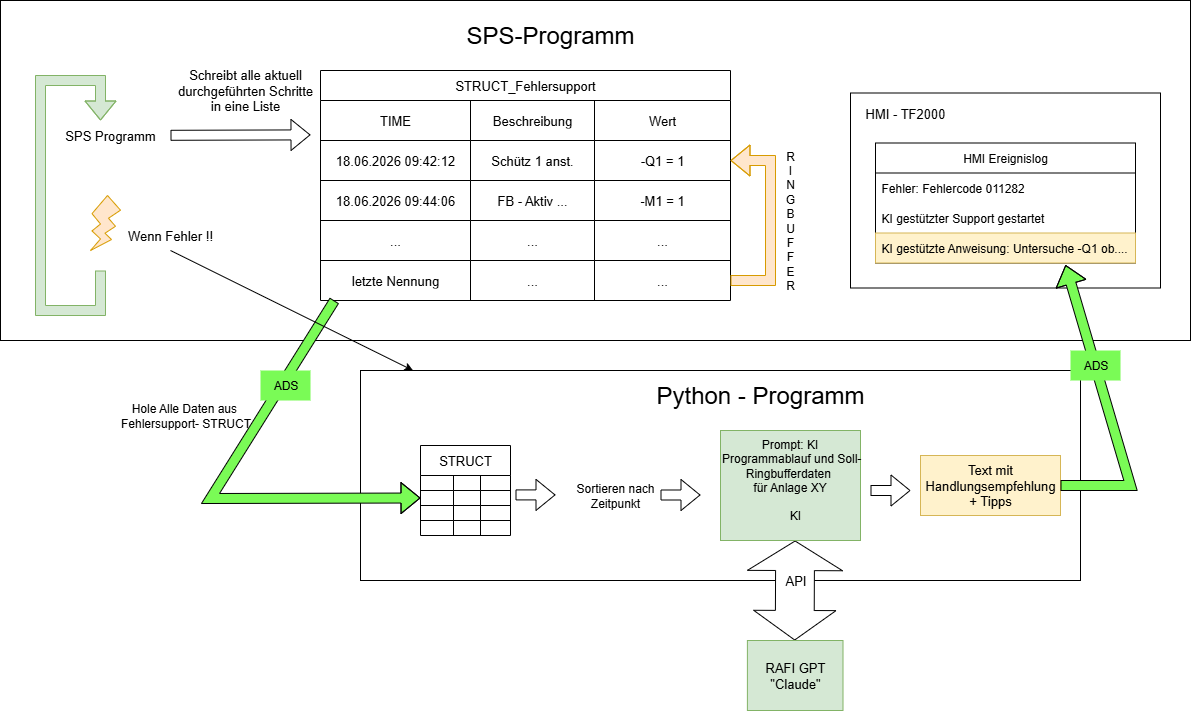
\includegraphics[width=\textwidth]{images/UmsetzungIntelligenterFehlersupport.drawio.png}
        \caption{Programmstruktur Intelligenter Fehlersupport}
        \label{fig:fehlersupport_ablauf}
        \end{figure}


    \subsubsection{Kontinuierliche Erfassung im Normalbetrieb}

        Im regulären Anlagenbetrieb werden Bedienereignisse, Anlagenzustände sowie Fehler- und Wartungseinträge fortlaufend in eine gemeinsame Ringpuffer-Datenstruktur als Array innerhalb des SPS-Programms geschrieben. Ein solcher Ringpuffer ist eine Datenspeicherstruktur, bei der nach Erreichen der letzten freien Speicherstelle der jeweils älteste Eintrag automatisch durch das neueste Element überschrieben wird. Das zugrundeliegende Prinzip ist in Abbildung~\ref{fig:ringbuffer} dargestellt.

        % Bild Ringbuffer
        \begin{figure}[H]
            \centering
            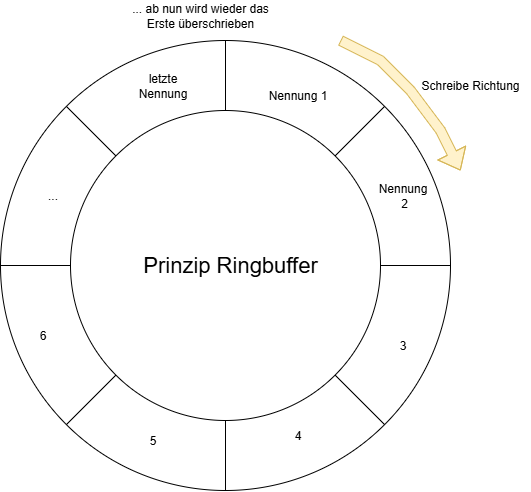
\includegraphics[width=\imgmedium]{images/RINGBUFFER.drawio.png}
            \caption{Prinzip des Ringpuffers}
            \label{fig:ringbuffer}
        \end{figure}

        Dadurch entsteht ein rollierender Datensatz der letzten Anlagenereignisse, in dem stets die zeitlich neuesten Vorgänge vorgehalten werden.
        
        Die Inhalte, die an bestimmten Programmstellen gespeichert werden sollen, sind dabei flexibel wählbar. Es wird jedoch empfohlen, alle aktorischen Elemente der Anlage durch aussagekräftige Beschreibungen zu erfassen. Auf diese Weise kann das System präzise angeben, welche Zylinder zu einem bestimmten Zeitpunkt beispielsweise ausgefahren sein müssten. Im Fehlerfall sieht das Personal sofort, ob diese Soll-Bedingung, also ob der Zylinder ausgefahren ist, erfüllt ist, wodurch sich die Fehlerursache schnell und zielgerichtet bestimmen lässt.

        Ebenso sollten regelmäßig aktive Programmschritte in den Speicher geschrieben werden, um bei Ablaufproblemen exakt nachvollziehen zu können, in welchem Produktionsschritt sich die Anlage gerade befindet. Darüber hinaus empfiehlt sich die Protokollierung verschiedener externer Einflüsse, wie etwa der zuvor genannten Ober- und Untergrenzen für den aktiven Druck im Pneumatiksystem. Ebenso sollten Bedienerinteraktionen erfasst werden, sprich gedrückter Knöpfe oder sonstiger Eingaben.

        Solange kein Fehler vorliegt, werden all diese Einträge fortlaufend durch neuere Daten überschrieben. Da sich die Anlage im produktiven Zustand befindet, ist dieser Datenverlust unkritisch, da kein Analysebedarf besteht. Spannend wird es hingegen, sobald die Anlage in einen Fehlerzustand wechselt.
    
    \subsubsection{Fehlerausgelöste Analysephase}

        Tritt an der Anlage ein Fehler auf, wird anlagenintern ein Fehlerbit gesetzt, auf das ein Mikrocomputer über OPC-UA reagieren kann. Auf diesem Mikrocomputer läuft ein Python-Skript, welches im ausgelösten Fall nacheinander die folgenden Schritte ausführt:

        \textbf{2.1 Auslesen der aktuellen Ringbufferinhalte:}

        Zunächst wird der vollständige Inhalt des Ringpuffers unmittelbar nach Auslösen des Fehlers aus der SPS-Steuerung über OPC-UA ausgelesen und an den Computer übermittelt.


        \textbf{2.2 Zeitliche Sortierung der Daten:}

        Im nächsten Schritt werden die ausgelesenen Daten im Python-Programm anhand ihrer Zeitstempel in eine chronologisch korrekte Reihenfolge gebracht. Dies ist notwendig, da aufgrund des Ringpufferprinzips zunächst keine lineare zeitliche Ordnung in den Rohdaten vorliegt. Mithilfe der Zeitstempel lässt sich diese Sortierung in Python jedoch problemlos umsetzen.

        \textbf{2.3 KI gestütztes Eingrenzen des Fehlers:}

        Das Python-Programm übermittelt die chronologisch sortierten Ereignisdaten per API an eine KI-Cloud. Entscheidend für die Qualität der anschließenden Auswertung ist ein präziser, vordefinierter System-Prompt, der dem KI-Modell den spezifischen Maschinenkontext vermittelt. Erst durch diese kontextuelle Grundlage ist das KI-System in der Lage, komplexe Zusammenhänge zwischen den verschiedenen Ereignissen zu erkennen und eine fundierte Einschätzung zur Fehlerursache zu formulieren. Darüber hinaus weist der System-Prompt die KI an, die ermittelte Ursache kompakt und verständlich in wenigen Sätzen für das Instandhaltungspersonal zusammenzufassen.

        \textbf{2.4 Darstellen der KI-Ergebnisse auf dem HMI-Display der Anlage:}

        Die Ausgabe des KI-Systems wird im Anschluss über die OPC-UA-Schnittstelle an das HMI übermittelt und dort in einem übersichtlichen Textfeld dargestellt. Die von der KI verfassten Sätze liefern dem Instandhaltungspersonal eine präzise Fehlerursache, eine entsprechende Eingrenzung sowie eine konkrete Handlungsempfehlung. Durch die direkte Visualisierung auf dem HMI-Display sind diese wertvollen Informationen für den Werker sofort abrufbar und im direkten Arbeitsumfeld anwendbar.
    \newpage
    

\section{Wirtschaftliche Gesamtbetrachtung und Rentabilität}

Um die Entscheidung für die Implementierung des neuen Systems fundiert zu begründen, werden in diesem Kapitel die Kosten des bisherigen Ausgangszustands den anfallenden Investitionen und Einsparungen des intelligenten Fehlersupports gegenübergestellt.

\subsection{Rahmenbedingungen und Annahmen}

Die Berechnung basiert auf einer typischen Produktionslinie im Zweischichtbetrieb mit folgenden Parametern:
\begin{itemize}
    \item \textbf{Betriebsdaten:} 220 Arbeitstage/Jahr, 3 Störungen/Tag $\implies$ \textbf{660 Fehlerfälle pro Jahr}.
    \item \textbf{Zeitersparnis durch Intelligenten Fehlersupport:} Reduzierung der Fehlersuchzeit um $10\,\text{Minuten}$ pro Störung (von 25 auf 15 Minuten).
    \item \textbf{Kostensätze:} Maschinenstundensatz $4{,}00\,\text{€/min}$ ($240\,\text{€/h}$); Instandhaltungspersonal $1{,}00\,\text{€/min}$ ($60\,\text{€/h}$).
    \item \textbf{KI-Token \& Daten:} Ringpuffer von $33.400\,\text{Zeichen}$ ($\approx 8.350\,\text{Input-Token}$) + Antwort von $560\,\text{Zeichen}$ ($\approx 140\,\text{Output-Token}$). 
    
    Preis: $\$3{,}00$ / Mio. Input-, $\$5{,}00$ / Mio. Output-Token:
    
    $\frac{8.350 \times \$3{,}00 + 140 \times \$5{,}00}{1.000.000} = \$0{,}02575 \approx \mathbf{\$0{,}03\,\text{bzw. } 0{,}03\,\text{€}}$ pro Fehlerfall.




    \item \textbf{Hardware \& Energie:} Computer im Dauerbetrieb ($15\,\text{W}$) bei $0{,}20\,\text{€/kWh}$.
\end{itemize}

\subsection{Laufende Betriebskosten}

Die laufenden Betriebskosten umfassen vor allem die variablen API-Tokengebühren für die Künstliche Intelligenz, sowie die Stromkosten der verwendeten Hardware:

\begin{itemize}
    \item \textbf{API-Tokenkosten:} $\$0{,}0258$ ($\approx 0{,}0237\,\text{€}$) pro Fehlerfall $\implies$ \textbf{$15{,}67\,\text{€/Jahr}$} bei 660 Aufrufen.
    \item \textbf{Energiekosten:} $15\,\text{W} \times 24\,\text{h} \times 365\,\text{Tage} = 131{,}4\,\text{kWh/Jahr} \implies \mathbf{26{,}28\,\text{€/Jahr}}$.
\end{itemize}

Die gesamten laufenden Betriebskosten betragen also: $15{,}67\,\text{€} + 26{,}28\,\text{€} = \mathbf{41{,}95\,\text{€/Jahr}}$.


\subsection{Erwartete Ersparnisse}

Demgegenüber steht der monetäre Jahresnutzen durch die Reduzierung der Stillstands- und Fehlersuchzeiten um kumuliert $6.600\,\text{Minuten/Jahr}$ ($110\,\text{Stunden}$):
\begin{align}
    \text{Ersparnis}_{\text{Produktion}} &= 6.600\,\text{min} \times 4{,}00\,\text{€/min} = 26.400{,}00\,\text{€/Jahr} \\
    \text{Ersparnis}_{\text{Personal}} &= 6.600\,\text{min} \times 1{,}00\,\text{€/min} = 6.600{,}00\,\text{€/Jahr}
\end{align}

Der Bruttonutzen beträgt somit $33.000{,}00\,\text{€/Jahr}$. Abzüglich der laufenden Betriebskosten ergibt sich eine Jahresersparnis von gesamt  $32.958{,}05\,\text{€}$.

\subsection{Investitionsaufwand}

Bevor von dieser Ersparnis profitiert werden kann, muss das System aber erst Implementiert werden. Für die Erstimplementierung fallen zunächst einmalige Investitionskosten an:

\begin{enumerate}
    \item \textbf{Hardwarebeschaffung:} Industrietauglicher Computer mit GPU: $1.500{,}00\,\text{€}$.
    \item \textbf{Engineering \& Integration:} Programmierung von SPS-Puffer, OPC-UA Gateway, HMI-Anbindung ($40\,\text{h}$ à $75\,\text{€/h}$): $3.000{,}00\,\text{€}$.
\end{enumerate}

\noindent Die einmalige Gesamtinvestition beträgt somit $\mathbf{ 4.500{,}00\,\text{€}}$.

\subsection{Amortisation}

Die Amortisationsdauer dieser Investition berechnet sich aus dem Verhältnis der einmaligen Investition zur jährlichen Ersparnis:
\[
    T_{\text{amort}} = \frac{\text{Investitionskosten}}{\text{Netto-Ersparnis}_{\text{Jahr}}} = \frac{4.500{,}00\,\text{€}}{32.958{,}05\,\text{€/Jahr}} \approx 0{,}137\,\text{Jahre} \approx \mathbf{1{,}6\,\text{Monate}}
\]

Bei der angenommenen Störungsfrequenz von 3 Störungen am Tag refinanziert sich das System bereits nach ca. 90 behobenen Fehlern vollständig. Somit ist dieses System eine sichere Investition. 

Folgende Grafik vergleicht die Kosten durch die Implementierung mit den Kosten, wenn die Implementierung nicht durchgeführt wird.

\begin{figure}[H]
        \centering
        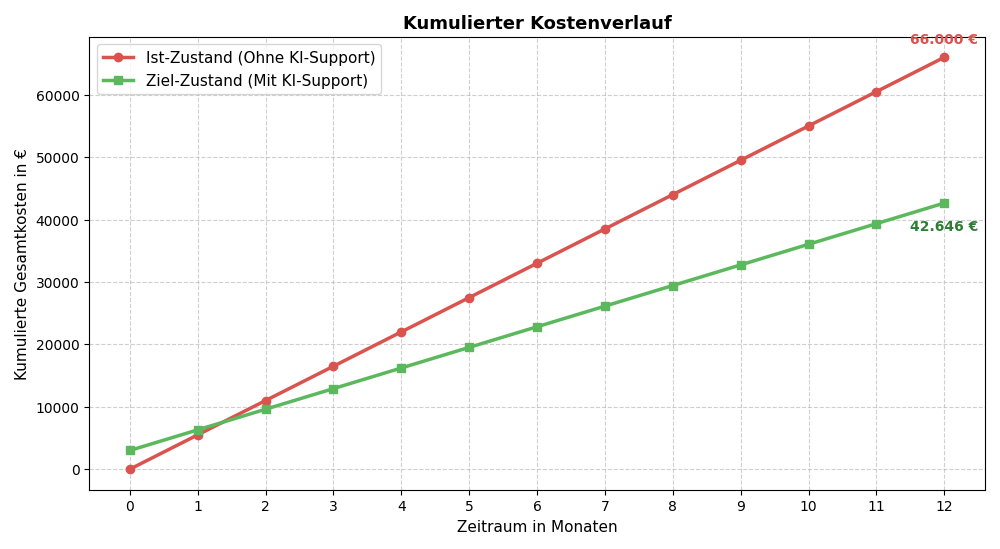
\includegraphics[width=\textwidth]{content/Code_um_Diagramme_darzustellen/Figure_1.png}
        \caption{Vergleich der Kostenentwicklungen bei Implementierung oder Belassen im Ausgangszustand}
        
        \end{figure}

\subsection{Fazit}
Mit einmaligen Investitionen von $4.500\,\text{€}$ und vernachlässigbaren Betriebskosten von unter $42\,\text{€/Jahr}$ weist das Konzept eine extrem kurze Amortisationszeit von unter zwei Monaten auf. Ab dem zweiten Betriebsmonat erwirtschaftet das System einen Netto-Vorteil von rund $33.000\,\text{€}$ pro Anlage und Jahr. Eine Umsetzung wird aus betriebswirtschaftlicher Sicht uneingeschränkt empfohlen.
    \newpage
    \section{Umsetzung und Risiken}

\subsection{Planung der Umsetzung}
Für die praktische Einführung des intelligenten Fehlersupports im industriellen Umfeld wird der strukturierte \textbf{PDCA-Zyklus} angewendet, um Ziele messbar zu erreichen und fortlaufend zu lernen:

\begin{itemize}[leftmargin=*, itemsep=2pt, parsep=0pt]
    \item \textbf{Plan (Planung):} Definition zentraler Ziele wie der spürbaren Reduktion von Stillstandszeiten und Entlastung der Instandhaltung. Festlegung messbarer Kennzahlen (z.\,B. Reparaturzeit-Reduktion um 30\,\%).
    \item \textbf{Do (Umsetzung):} Schrittweise Implementierung einer Testanlage. Beschaffung eines passenden Computers mit GPU, Programmierung der SPS-Schnittstelle für den Ringspeicher sowie Entwicklung der Python-Schnittstelle zur Kommunikation mit der KI.
    \item \textbf{Check (Überprüfung):} Mehrwöchiger Test im Schichtbetrieb. Abgleich der Ist-Werte mit historischen Stillstandszeiten, Überprüfung des Zeitersparnisses (Ziel: ca. 10 Min./Störung) und Einhaltung des Budgets von ca. 40 Arbeitsstunden.
    \item \textbf{Act (Standardisierung):} Nach erfolgreicher Testphase erfolgt die Übernahme in die RAFI-Richtlinien. Künftige Neuanlagen werden direkt ab Werk ausgestattet, Bestandsanlagen schrittweise nachgerüstet.
\end{itemize}

\subsection{Stakeholder und Abhängigkeiten der Umsetzung}
Für eine erfolgreiche Umsetzung müssen verschiedene Stakeholder eng zusammenarbeiten. 
Die Beteiligten und der Ablauf hängen dabei direkt voneinander ab, da einzelne Phasen zwingend aufeinander aufbauen.
Deshalb ist das Projekt nur zielführend wenn versvchiedene Akteure koordiniert zusammenarbeiten. 
Dieses Kapitel beschäftigt sich mit dieser Koordination. 

Der Prozess startet im \textbf{Einkauf}, der für die Beschaffung der erforderlichen Hardware, also des Computers und der GPU, zuständig ist. 
Zum Identifizieren von geeigneten Bauteilen wird ein Elektroingenuer der Automatisierungsabteilung zur Verfügung gestellt. 

Erst wenn die Hardware vorliegt, können die \textbf{Programmierer und die Softwareentwicklung} mit der praktischen Arbeit beginnen.
Sie richten die Schnittstellen in der SPS ein, programmieren den Ringpuffer und binden die Python-Schnittstelle zur KI-Cloud an. 
Die Programmierung und Validierung auf der Testanlage ist wiederum die Voraussetzung für die nächste Phase.

Nach erfolgreicher technischer Umsetzung erfolgt die Übergabe an die \textbf{Produktion und das Instandhaltungspersonal}. 
Dieser Schritt umfasst eine gründliche Einweisung der Mitarbeiter vor Ort, damit diese die KI-gestützten Rückmeldungen auf 
dem HMI-Display im Arbeitsalltag richtig deuten und nutzen können. Das Feedback der Werker dient abschließend dazu,
das System feinzujustieren und den dauerhaften Betrieb sicherzustellen. Das ist auch im Sinne des des kontinuierlichen Verbesserungsprozesses KVP.

\subsection{Einzugehende Risiken}

\subsubsection*{Finanzielles Risiko der Investition}
Das finanzielle Risiko ist durch eine geringe Anfangsinvestition von rund 4.500\,€ minimal und vollkommen überschaubar. Selbst bei geringerer Zeitersparnis (z.\,B. 3--4 statt 10 Minuten) verlängert sich lediglich die Amortisationszeit von rund zwei auf fünf bis sechs Monate. Da die laufenden Betriebskosten bei ca. 3\,Cent pro Störung liegen und keine teuren Wartungsverträge anfallen, entstehen keine unkontrollierbaren Folgekosten. Der angeschaffte Computer mit GPU ist zudem flexibel anderweitig nutzbar.

\subsubsection*{Risiko der Datensicherheit im Umgang mit künstlichen Intelligenzen}
Um den Schutz von Firmengeheimnissen zu gewährleisten, werden ausschließlich technische Messwerte (Ströme, Temperaturen, Fehlernummern) übermittelt. Sensible Produktionsdaten, Rezepturen oder Mitarbeiterdaten verbleiben im Unternehmen. Zusätzlich reglementiert ein strenger System-Prompt das KI-Modell, sodass dieses thematisch fokussiert bleibt.


    \newpage
    \section{Zusammenfassung und Entscheidungsvorlage}

Wenn eine moderne Produktionsanlage stehen bleibt, führt die herkömmliche Fehlersuche zu zeitraubenden Suchen von Maschinendaten und komplexen Analysen von Signalzuständen. 

Das in dieser Arbeit vorgestellte Konzept löst dieses Problem durch einen intelligenten Fehlersupport: Die Steuerung speichert im funktionsfähigem Zustand Aktionen und Messwerte in einem Ringspeicher.
Im Fehlerfall  werden die Daten automatisch von einer Künstlichen Intelligenz analysiert. Die KI zeigt dem Techniker Ursache und Behebung des Fehlers direkt auf dem HMI-Bedienbildschirm an.

Dadurch verkürzt sich die Stillstandszeit um durchschnittlich zehn Minuten pro Fehlerfall. Bei einmaligen Entwicklungskosten von rund 4.500 Euro spart das System über 26.000 Euro pro Jahr ein und amortisiert sich nach rund zwei Monaten.

\subsection{Entscheidungsfrage}
Soll das Konzept für den intelligenten Fehlersupport genehmigt, im Rahmen eines Studentenprojekts an einer realen Produktionslinie getestet und bei nachgewiesenem Erfolg als neuer Standard für alle weiteren Anlagen bei RAFI eingeführt werden?

\subsection{Konkrete Entscheidungsvorlage für das Management}
Dem Management wird empfohlen, das Budget von 4.500 Euro freizugeben, um das System innerhalb von acht Wochen an einer Testanlage in Betrieb zu nehmen. Während dieser Phase soll überprüft werden, ob die Reparaturzeiten um mindestens 25 Prozent sinken und die Praxistauglichkeit gegeben ist. Bei Erfolg wird die Lösung fest in den RAFI-Standard übernommen. Das Management beschließt damit, die Digitalisierung der Fertigung voranzutreiben, ungeplante Stillstände zu reduzieren und die Wirtschaftlichkeit nachhaltig zu steigern.
    \newpage
    %Abbildungsverzeichnis -----------------------------------------------------------------------------------------
    \pagenumbering{Roman}
    %\setcounter{page}{\value{savepage}+1}
    %\listoffigures

    %Formelzeichenverzeichnis---------------------------------------------------------------------------------------
    %\newpage
    %\input{content/100_Formelzeichen.tex}
    
    

    %Abkürzungsverzeichnis------------------------------------------------------------------------------------------
    %\newpage
    %\input{content/101_Abkuerzungsverzeichnis.tex}

    %Tabellenverzeichnis--------------------------------------------------------------------------------------------
    %\newpage
    %\listoftables

    %Nutzung künstlicher Intelligenzen------------------------------------------------------------------------------
    \newpage
    \section*{Nutzung künstlicher Intelligenzen}
In folgender Tabelle werden verschiedene KI-Werkzeuge und deren Nutzung in Verbindung mit dieser Arbeit beschrieben. Durch den Einsatz dieser KI-Werkzeuge konnte die Arbeitseffizienz gesteigert werden.

\begin{tabular}{|p{2.2cm}|p{9.5cm}|p{3.5cm}|}
  \hline
  \textbf{Werkzeug} & \textbf{Beschreibung der Nutzung} & \textbf{Arbeitsschritt / Kapitel} \\
  \hline
  \multicolumn{3}{|l|}{\textbf{1. Allgemein}} \\
  \hline
  ChatGPT/ RAFIGPT (Claude)/ Gemini & Verschaffen eines Überblicks über Inhalte und Vorgehen in diesem Projekt. & Planung \\
  \hline
  \multicolumn{3}{|l|}{\textbf{2. Konzeption des Intelligenten Fehlersupports}} \\
  \hline
  RAFI-GPT (Claude) &
  Unterstützung bei der PLanung und Konzeptionierung des Lösungskonzepts. &
  Erstellung Konzept \\
  \hline
  \multicolumn{3}{|l|}{\textbf{3. Erstellen der Dokumentation}} \\
  \hline
  ChatGPT & Unterstützung beim Umgang mit VS-Code & Dokumentation \\
  \hline
  GitHub Copilot & Unterstützung beim Verfassen einzelner Formulierungen sowie bei der Korrektur von Rechtschreibfehlern & Dokumentation\\
  \hline
  ChatGPT & Unterstützung bei Latex und Analyse von Compilerfehlern & Dokumentation \\
  \hline
\end{tabular}










    %Literaturverzeichnis-------------------------------------------------------------------------------------------
    \newpage
    \printbibliography
\end{document}